\documentclass{chi-ext}
% Please be sure that you have the dependencies (i.e., additional LaTeX packages) to compile this example.
% See http://personales.upv.es/luileito/chiext/

\copyrightinfo{
  Copyright is held by the author/owner(s).\\
  \emph{CHI'13}, April 27 -- May 2, 2013, Paris, France.\\
  ACM 978-1-XXXX-XXXX-X/XX/XX.\\
}

\title{Using Distributed Information Stores for Patient-Clinician Health Data Sharing}

\numberofauthors{3}
% Notice how author names are alternately typesetted to appear ordered in 2-column format;
% i.e., the first 4 autors on the first column and the other 4 auhors on the second column.
% Actually, it's up to you to strictly adhere to this author notation.
\author{
  \vspace{-1.5em} % lisatolles: The abstract heading should start at the time height on the page as the authors names
  \alignauthor{
  	\textbf{Daniel A. Smith}\\
  	\affaddr{Web and Internet Science Research Group}\\
%  	\affaddr{Electronics and Computer Science}\\
  	\affaddr{University of Southampton}\\
  	\affaddr{Southampton, UK}\\
  	\email{ds@ecs.soton.ac.uk}
  }\alignauthor{
  	\textbf{Max Van Kleek}\\
  	\affaddr{Web and Internet Science Research Group}\\
%  	\affaddr{Electronics and Computer Science}\\
  	\affaddr{University of Southampton}\\
  	\affaddr{Southampton, UK}\\
  	\email{emax@ecs.soton.ac.uk}
  }
  \vfil
  \alignauthor{
  	\textbf{Nigel R. Shadbolt}\\
  	\affaddr{Web and Internet Science Research Group}\\
%  	\affaddr{Electronics and Computer Science}\\
  	\affaddr{University of Southampton}\\
  	\affaddr{Southampton, UK}\\
  	\email{nrs@ecs.soton.ac.uk}
  }
  \vfil
  \vfil
  \vfil
  \vfil
}

% Paper metadata (use plain text, for PDF inclusion and later re-using, if desired)
\def\plaintitle{Using Distributed Information Stores for Patient-Clinician Health Data Sharing}
\def\plainauthor{Daniel A. Smith, Max Van Kleek, Nigel R. Shadbolt}
\def\plainkeywords{personal data, patient care, healthcare, information stores}
\def\plaingeneralterms{Personal Data, Patient Care, Healthcare, Information Stores}

\hypersetup{
  % Your metadata go here
  pdftitle={\plaintitle},
  pdfauthor={\plainauthor},  
  pdfkeywords={\plainkeywords},
  pdfsubject={\plaingeneralterms},
  % Quick access to color overriding:
  %citecolor=black,
  %linkcolor=black,
  %menucolor=black,
  %urlcolor=black,
}


\usepackage{graphicx}   % for EPS use the graphics package instead
\usepackage{balance}    % useful for balancing the last columns
\usepackage{bibspacing} % save vertical space in references

\usepackage{url}

\begin{document}

\maketitle

\begin{abstract}

Existing approaches to electronic integrated health records have largely focused on centralised information architectures, where patient data is held in a single repository, and accessed over the internet. However, there are a number of benefits to both patients and clinicians in a decentralised information approach to health records.

\end{abstract}

\keywords{\plainkeywords}
%\textcolor{red}{Mandatory section to be included in your final version.}

\category{H.5.m}{Information interfaces and presentation (e.g., HCI)}{Miscellaneous}. 
%See \cite{ACMCCS} 
%See: \url{http://www.acm.org/about/class/1998/} 
%or help using the ACM Classification system.
%\textcolor{red}{Mandatory section to be included in your final version.}

%\terms{\plaingeneralterms}
%\textcolor{red}{Optional section to be included in your final version.}


\section{Introduction}

A key goal in improving patient-clinician communication is
establishing a common context for communication with which a shared
understanding can be established.  This understanding is
bi-directional, in the sense that the patient needs to be able to
effectively interpret what the clincian is trying to convey to him or
her, but also the clinician needs to be able to arrive at an accurate
characterisation of the patient's situation (often under time
constraints) as updated since the last time the clinician met with the
patient.

One of the most promising technologies that has the potential to help
provide such a common context is the patient-centric electronic health
record (henceforth EHR)\cite{ehr}, a digital representation of the
complete medical history of an individual as recorded by clinicians
throughout a patient's life. The EHR promises to enable both
patients and their clinicians unfettered access to the patient's
medical data, including diagnostics, reports, and history of
interventions.  This means that clinicians can more easily review a
patient's long-term history in the course of basing interpretations
and interventions. Moreover, since patients have access to their own
medical histories, there is (theoretically) a basis by which patients
can understand the justifications for clinicial prognoses.

% proactive activity recording to provide sketches of a person's
% activity profiles outside of the hospital, streaming data

Yet so far, the ``medical history'' that EHRs have been used to store
have constituted only the official diagnoses and diagnostic reports
prepared by clinicians, technicians and nurses


% challenges to 
% background on authors
% 


\section{Personal Electronic Sensors}

There has been a surge in popularity of personal electronic sensors as
part of the ``quantified-self'' movement to measure and improve one's health.
Wireless sensors such as the Fit-bit and Nike FuelBand and small and discreet,
yet provide the wearer with a wealth of information about their own activity level.
In particular, wearers have a desire to improve their health and fitness, based on
the feedback they receive from their device.

The measurements from such devices are of particular interest because of the
frequency and granularity of measurement that they perform - showing minute-by-minute updates
throughout the day, with no clinical involvement. 

In addition to fitness monitors, the market for quantified self sensors has
expanded into areas of personal health. For example, there are sensors for
measuring blood oxygenation\footnote{SpO2 Blood Oxygenation sensor: \url{http://ispo2.com}},
Heart Rate Variability and Respiratory Rate\footnote{Zensorium Tinke, heart and respiratory rate sensor: \newline \indent \indent \indent \url{http://www.zensorium.com/tinke/}} and
Temperature and Galvanic Skin Response\footnote{BodyMedia Core 2, temperature and GSR sensor: \newline \indent \indent \indent  \url{http://www.bodymedia.com}}.
The diet aspect of weight loss is also covered, by products such as a wireless fork that informs you how long you spent eating\footnote{HapiLabs HapiFork: \newline \indent \indent \indent  \url{http://hapilabs.com/products-hapifork.asp}}.

Currently these products tend to work in isolation, where the readings from a single product
are presented either on the device themselves, or via a smartphone or website. However,
their use could be integrated with clinical care, in order to monitor patients, and to give an
insight into their lifestyle.




%% =============================================================================
%\section{Introduction}
%% =============================================================================
%This format is to be used for submissions that are published in the conference extended abstracts.  
%We wish to give this volume a consistent, high-quality appearance. 
%We therefore ask that authors follow some simple guidelines. 
%In essence, you should format your paper exactly like this document. 
%The easiest way to do this is simply to download a template from the conference website and replace the content with your own material.
%
%% =============================================================================
%\section{Copyright}
%% =============================================================================
%For publications in the CHI Extended Abstracts, copyright remains with the author.  
%The publication is not considered an archival publication; however, it does go into the ACM Digital Library. 
%Because you retain copyright, as the author you are free to use this material as you like, including submitting a paper based on this work to other conferences or journals.  
%Authors grant unrestricted permission for ACM to publish the accepted submission in the CHI Extended Abstracts without additional consideration or remuneration.
%
%% =============================================================================
%\section{Text formatting}
%% =============================================================================
%Please use an 8.5-point Verdana font, or other sans serifs font as close as possible in appearance to Verdana in which these guidelines have been set. 
%Arial 9-point font is a reasonable substitute for Verdana as it has a similar x-height. 
%Please use serif or non-proportional fonts only for special purposes, such as distinguishing source code text.
%Additionally, here is an example of footnoted text.\footnote{Use footnotes sparingly, if at all.}
%As stated in the footnote, footnotes should rarely be used.
%
%\subsection{Language, style, and content}
%% -----------------------------------------------------------------------------
%The written and spoken language of SIGCHI is English. 
%Spelling and punctuation may use any dialect of English (e.g., British, Canadian, US, etc.) provided this is done consistently. 
%Hyphenation is optional. 
%To ensure suitability for an international audience, please pay attention to the following:
%
%\begin{itemize}\compresslist
%\item 	
%Write in a straightforward style. 
%Use simple sentence structure. 
%Try to avoid long sentences and complex sentence structures. 
%Use semicolons carefully.
%\item 	
%Use common and basic vocabulary (e.g., use the word ``unusual" rather than the word ``arcane").
%\item 	
%Briefly define or explain all technical terms. 
%The terminology common to your practice/discipline may be different in other design practices/disciplines.
%\item 	
%Spell out all acronyms the first time they are used in your text. 
%For example, ``World Wide Web (WWW)".
%\item 	
%Explain local references (e.g., not everyone knows all city names in a particular country).
%\item 	
%Explain ``insider" comments. 
%Ensure that your whole audience understands any reference whose meaning you do not describe (e.g., do not assume that everyone has used a Macintosh or a particular application).
%\item 	
%Explain colloquial language and puns. 
%Understanding phrases like ``red herring" requires a cultural knowledge of English. 
%Humor and irony are difficult to translate.
%\item 	
%Use unambiguous forms for culturally localized concepts, such as times, dates, currencies and numbers (e.g., ``1-5-97" or ``5/1/97" may mean 5 January or 1 May, and ``seven o'clock" may mean 7:00 am or 19:00).
%\item 	
%Be careful with the use of gender-specific pronouns (he, she) and other gender-specific words (chairman, manpower, man-months). 
%Use inclusive language (e.g., she or he, they, chair, staff, staff-hours, person-years) that is gender-neutral. 
%If necessary, you may be able to use ``he" and ``she" in alternating sentences, so that the two genders occur equally often~\cite{Schwartz95}. 
%\end{itemize}
%
%
%% =============================================================================
%\section{Figures}
%% =============================================================================
%The examples on this and following pages should help you get a feel for how screen-shots and other figures should be placed in the template. 
%Be sure to make images large enough so the important details are legible and clear.
%
%%\begin{figure}
%%  \centering
%%  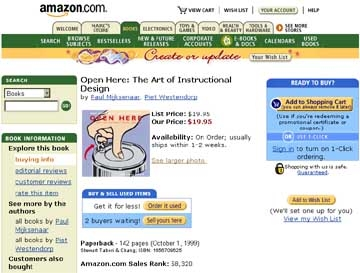
\includegraphics[width=\linewidth]{sample.jpg}
%%  \caption{Insert a caption below each figure.}
%%  \label{fig:sample}
%%\end{figure}
%
%Your document may use color figures, which are included in the page limit; the figures must be usable when printed in black and white.
%You can use the \LaTeX's \texttt{marginpar} command to insert figures in the (right) margin side of the document (see \autoref{fig:marginparsample}).
%
%
%% =============================================================================
%\section{References and Citations}
%% =============================================================================
%Use a numbered list of references at the end of the article, ordered alphabetically by first author, and referenced by numbers in brackets \cite{Anderson92,Klemmer02,Mather00,Zellweger01}
%For papers from conference proceedings, include the title of the paper and an abbreviated name of the conference (e.g., for Interact 2003 proceedings, use Proc. Interact 2003). 
%Do not include the location of the conference or the exact date; do include the page numbers if available. 
%See the examples of citations at the end of this document. 
%
%Your references should be published materials accessible to the public.  
%Internal technical reports may be cited only if they are easily accessible (i.e., you provide the address for obtaining the report within your citation) and may be obtained by any reader for a nominal fee.  
%Proprietary information may not be cited. 
%Private communications should be acknowledged in the main text, not referenced  (e.g., [Robertson, personal communication]).
%
%
%% =============================================================================
%\section{Producing and testing PDF files}
%% =============================================================================
%We recommend that you produce a PDF version of your submission well before the final deadline. 
%Besides making sure that you are able to produce a PDF, you will need to check that (a) the length of the file remains within the submission category's page limit, (b) the PDF file size is 4 megabytes or less, and (c) the file can be read and printed using Adobe Acrobat Reader. 
%Test your PDF file by viewing or printing it with the same software we will use when we receive it, Adobe Acrobat Reader Version 7. 
%This is widely available at no cost from~\cite{Acrobat7}.  
%Note that most reviewers will use a North American/European version of Acrobat reader, which cannot handle documents containing non-North American or non-European fonts (e.g. Asian fonts).  
%Please therefore do not use Asian fonts, and verify this by testing with a North American/European Acrobat reader (obtainable as above). Something as minor as including a space or punctuation character in a two-byte font can render a file unreadable.
%
%
%% =============================================================================
%\section{Dummy text}
%% =============================================================================
%Lorem ipsum dolor sit amet, consectetur adipiscing elit. Duis ut eros semper lectus vehicula elementum. Vestibulum ante ipsum primis in faucibus orci luctus et ultrices posuere cubilia Curae; Aliquam quis mi sapien. Suspendisse potenti. Mauris ultrices euismod velit sed dictum. Nullam auctor, nulla tincidunt dapibus suscipit, velit leo convallis metus, vel commodo libero erat in dolor. In laoreet porttitor ligula, porta blandit lectus consequat quis. 
%
%Nam ut eros dui. Mauris volutpat elit metus, euismod pellentesque purus. In hac habitasse platea dictumst. Nullam consectetur lacinia interdum. Sed nec blandit nisi. Proin in nulla purus, sit amet iaculis tortor. Ut dapibus pellentesque nulla in interdum. Nunc at velit felis. Curabitur euismod neque eu orci varius in pharetra sem interdum. Morbi in mauris ac risus iaculis dapibus id in magna. Class aptent taciti sociosqu ad litora torquent per conubia nostra, per inceptos himenaeos.
%
%%\marginpar{
%%\begin{figure}
%%  \begin{center}
%%  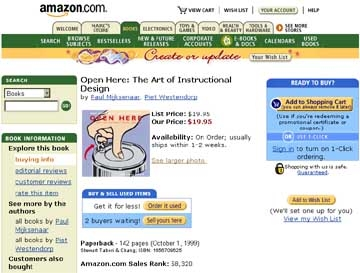
\includegraphics[width=\marginparwidth]{sample.jpg}
%%  \caption{A marginal figure.}
%%  \label{fig:marginparsample}
%%  \end{center}  
%%\end{figure}
%%}
%
%Aliquam consectetur quam sed odio varius vitae rhoncus urna fermentum. Phasellus viverra diam non justo porttitor varius. Integer ultrices accumsan lectus eget mollis. Nulla et leo sit amet nunc ornare rutrum sit amet ac dui. Cras vehicula accumsan purus nec fermentum. Mauris viverra condimentum metus, ut posuere quam laoreet nec. Phasellus massa tellus, ullamcorper nec porta sed, aliquet vitae nulla. Phasellus non tortor mauris. Cras ullamcorper egestas erat, vel rutrum elit viverra a. Donec in nisl ut est facilisis blandit. Quisque congue accumsan risus, ut venenatis magna vulputate vel. Nam commodo sapien vel mauris adipiscing nec dictum quam congue. Phasellus tempor vestibulum nisl quis blandit. Nullam condimentum auctor nibh, quis elementum libero tristique.



%\section{Acknowledgements}
%We thank all DUX 2003 publications support and staff who wrote this document originally and allowed us to modify it for this conference.
%This template was based on Manas Tungare's \texttt{chi.cls}, and rewritten by Luis A. Leiva.

\balance
\bibliographystyle{acm-sigchi}
\bibliography{sample}

\end{document}
